\chapter{Deployment}
Development of our application was performed locally using \textbf{docker-compose} to glue up 4 components necessary to sufficiently orchestrate \underline{PHP container} for web application with \underline{MySQL container} (+ \underline{Adminer container}) and \underline{Redis container}.
\par
We have to, however, run our application in \textbf{Kubernetes Cluster}. \textbf{Services} and \textbf{Deployments} have to be written. Services for the purpose of routing and taking care of new container spawn addresses. Deployments to describe container definitions - images \& volumes, number of replicas and environment variables. \textbf{Database} is run as a separate standalone entity within the cluster with persistent storage, \textbf{Redis} for syncing and preserving sessions as well.
\newline
\par
\section*{SwimmPair running in the Kubernetes Cluster}
\par
\begin{figure}[h]
    \centering	
    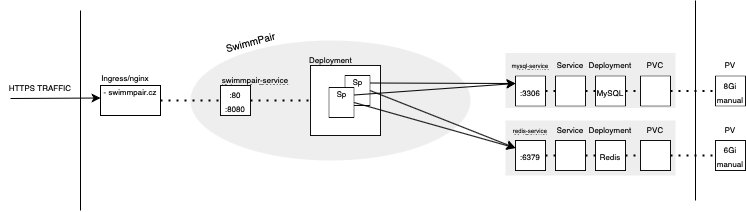
\includegraphics[scale=0.52]{img/swimmpair_deployment_k8s.png}
    \caption{Preview of our Kubernetes setup with running application.}
    \label{fig5.1:deplk8s}
\end{figure}
Both \textbf{Database} and \textbf{Redis} can be substituted by Managed Databases\footnote{\url{https://www.digitalocean.com/products/managed-databases}} or their equivalents in different cloud providers. They can be accessed remotely as dedicated self-hosted services within your own company as well.
\par \textbf{SwimmPair} can be run in some Container Services or "1-click apps" as well. 
\section*{Dockerization of SwimmPair application}
A file called \textbf{Dockerfile} has to be ready in the project folder.
\begin{lstlisting}
FROM thecodingmachine/php:7.4-v4-apache
COPY --chown=docker . /var/www/html
\end{lstlisting}
This image of PHP7.4/Apache\footnote{Image \textbf{thecodingmachine/php:7.4-v4-apache}  by TheCodingMachine - \url{https://github.com/thecodingmachine/docker-images-php}} was chosen because it correctly dockerizes part of so-called "LAMP stack". In order to build this image and push it into Docker Hub we need to run these following commands:
\begin{lstlisting}
docker build -t stepanklos/swimmpair .
docker push stepanklos/swimmpair
\end{lstlisting}
This image is then pullable as stepanklos/swimmpair:latest\footnote{\url{https://hub.docker.com/repository/docker/stepanklos/swimmpair/general}} by K8s Deployment.
\section*{Kubernetes}
We run two replicas on two nodes to ensure reliability and uptime. Additionally, we have set up an autoscaler to accommodate future increases in traffic.
\subsection*{Kubernetes autoscaler for increased workloads}
\begin{figure}[h]
    \centering	
    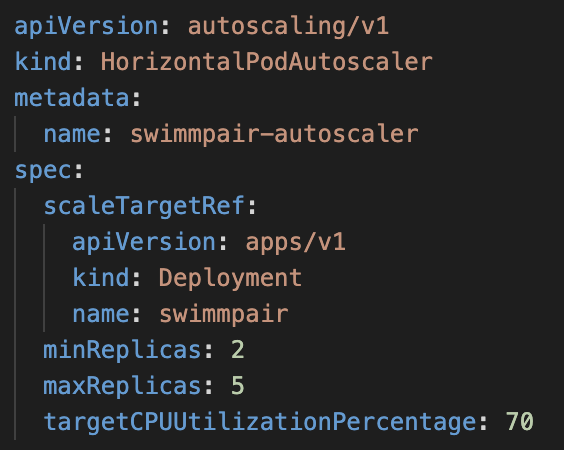
\includegraphics[scale=0.52]{img/swimmpair_deloyment_k8s_scaling.png}
    \caption{Autoscaler for Deployment to accomodate larger application traffic.}
    \label{fig5.2:k8sautoscaling}
\end{figure}
\subsection*{Deployment app-swimmpair.yaml}
\begin{lstlisting}
apiVersion: apps/v1
kind: Deployment
metadata:
  name: swimmpair
spec:
  replicas: 2
  selector:
    matchLabels:
      app: swimmpair
  template:
    metadata:
      labels:
        app: swimmpair
    spec:
      containers:
      - name: swimmpair
        image: stepanklos/swimmpair:latest
        securityContext:
          allowPrivilegeEscalation: true
        ports:
        - containerPort: 80
        env:
        - name: MESSAGE
          value: Hello from swimmpair Deployment!
        - name: DATABASE_HOST
          value: 'mysql-service'
        - name: DATABASE_USER
          value: 'root'
        - name: DATABASE_PASS
          value: 'heslo'
        - name: DATABASE_NAME
          value: 'plavani' 
        - name: PHP_INI_SESSION__SAVE_HANDLER
          value: 'redis'
        - name: PHP_INI_SESSION__SAVE_PATH
          value: 'tcp://redis-service:6379?auth=aGVzbG8='
\end{lstlisting}    
\section*{Database and Redis}
As mentioned, our application does not come with a database (and Adminer) or Redis, so we had to set them up separately using a PV (Persistent Volume) on which a PVC (Persistent Volume Claim) was created. Due to Digital Ocean's policy on PersistentVolume implementation, we had to run these services as 1 pod with manual volume, which is completely sufficient for our workload.
\newline
These two services we set up are internally accessible as follows:
\begin{itemize}
    \item MySQL Database\footnote{\url{https://github.com/KlosStepan/DOKS-configs/tree/main/mysql-deployment}}: \textbf{mysql-service:3306},
    \item \textbf{Re}mote \textbf{Di}ctionary \textbf{S}erver: \footnote{\url{https://github.com/KlosStepan/DOKS-configs/tree/main/redis-deployment}} \textbf{redis-service:6379},
\end{itemize}
in our Kubernetes Cluster.
